\section{Introduction}
\label{sec:intro}
Suppose a transport planner wants to know how passengers would respond to a less reliable bus service. A model might reproduce today's public-transport share and still predict the wrong change tomorrow. It might also predict a reasonable change that disappears when travelers are assigned to routes and vehicles. Scenario analysis therefore needs more than an accurate baseline: it needs a defensible account of how choices change and how those changes reach the network \citep{horni2016multi}.

Large language models (LLMs) offer a flexible way to describe such choices. They can combine a traveler's circumstances with trip attributes and contextual information in a single prompt. Recent work uses this capacity for travel prediction, route choice and agent-based modeling \citep{mo2026llmtravel,wang2025agentic,liu2025framework}. Repeatedly querying an LLM for a simulated population is costly, however. Behavioral distillation addresses this problem by fitting a compact local model, the \emph{Student}, to judgments elicited from an LLM, the \emph{Teacher}. The Student can then generate travel choices without a live LLM call for every decision.

What should survive this compression? Conventional evaluation asks whether the Student matches the Teacher at individual input states. Transport scenario analysis also asks whether it preserves the change between two states: the same person making the same trip under different conditions. We call the first property \emph{static fidelity} and the second \emph{response fidelity}. Exact agreement at every state would imply exact agreement in every response. With limited data and model capacity, an average static score does not directly assess the particular changes a planner needs.

\begin{figure}[pos=htbp]
\centering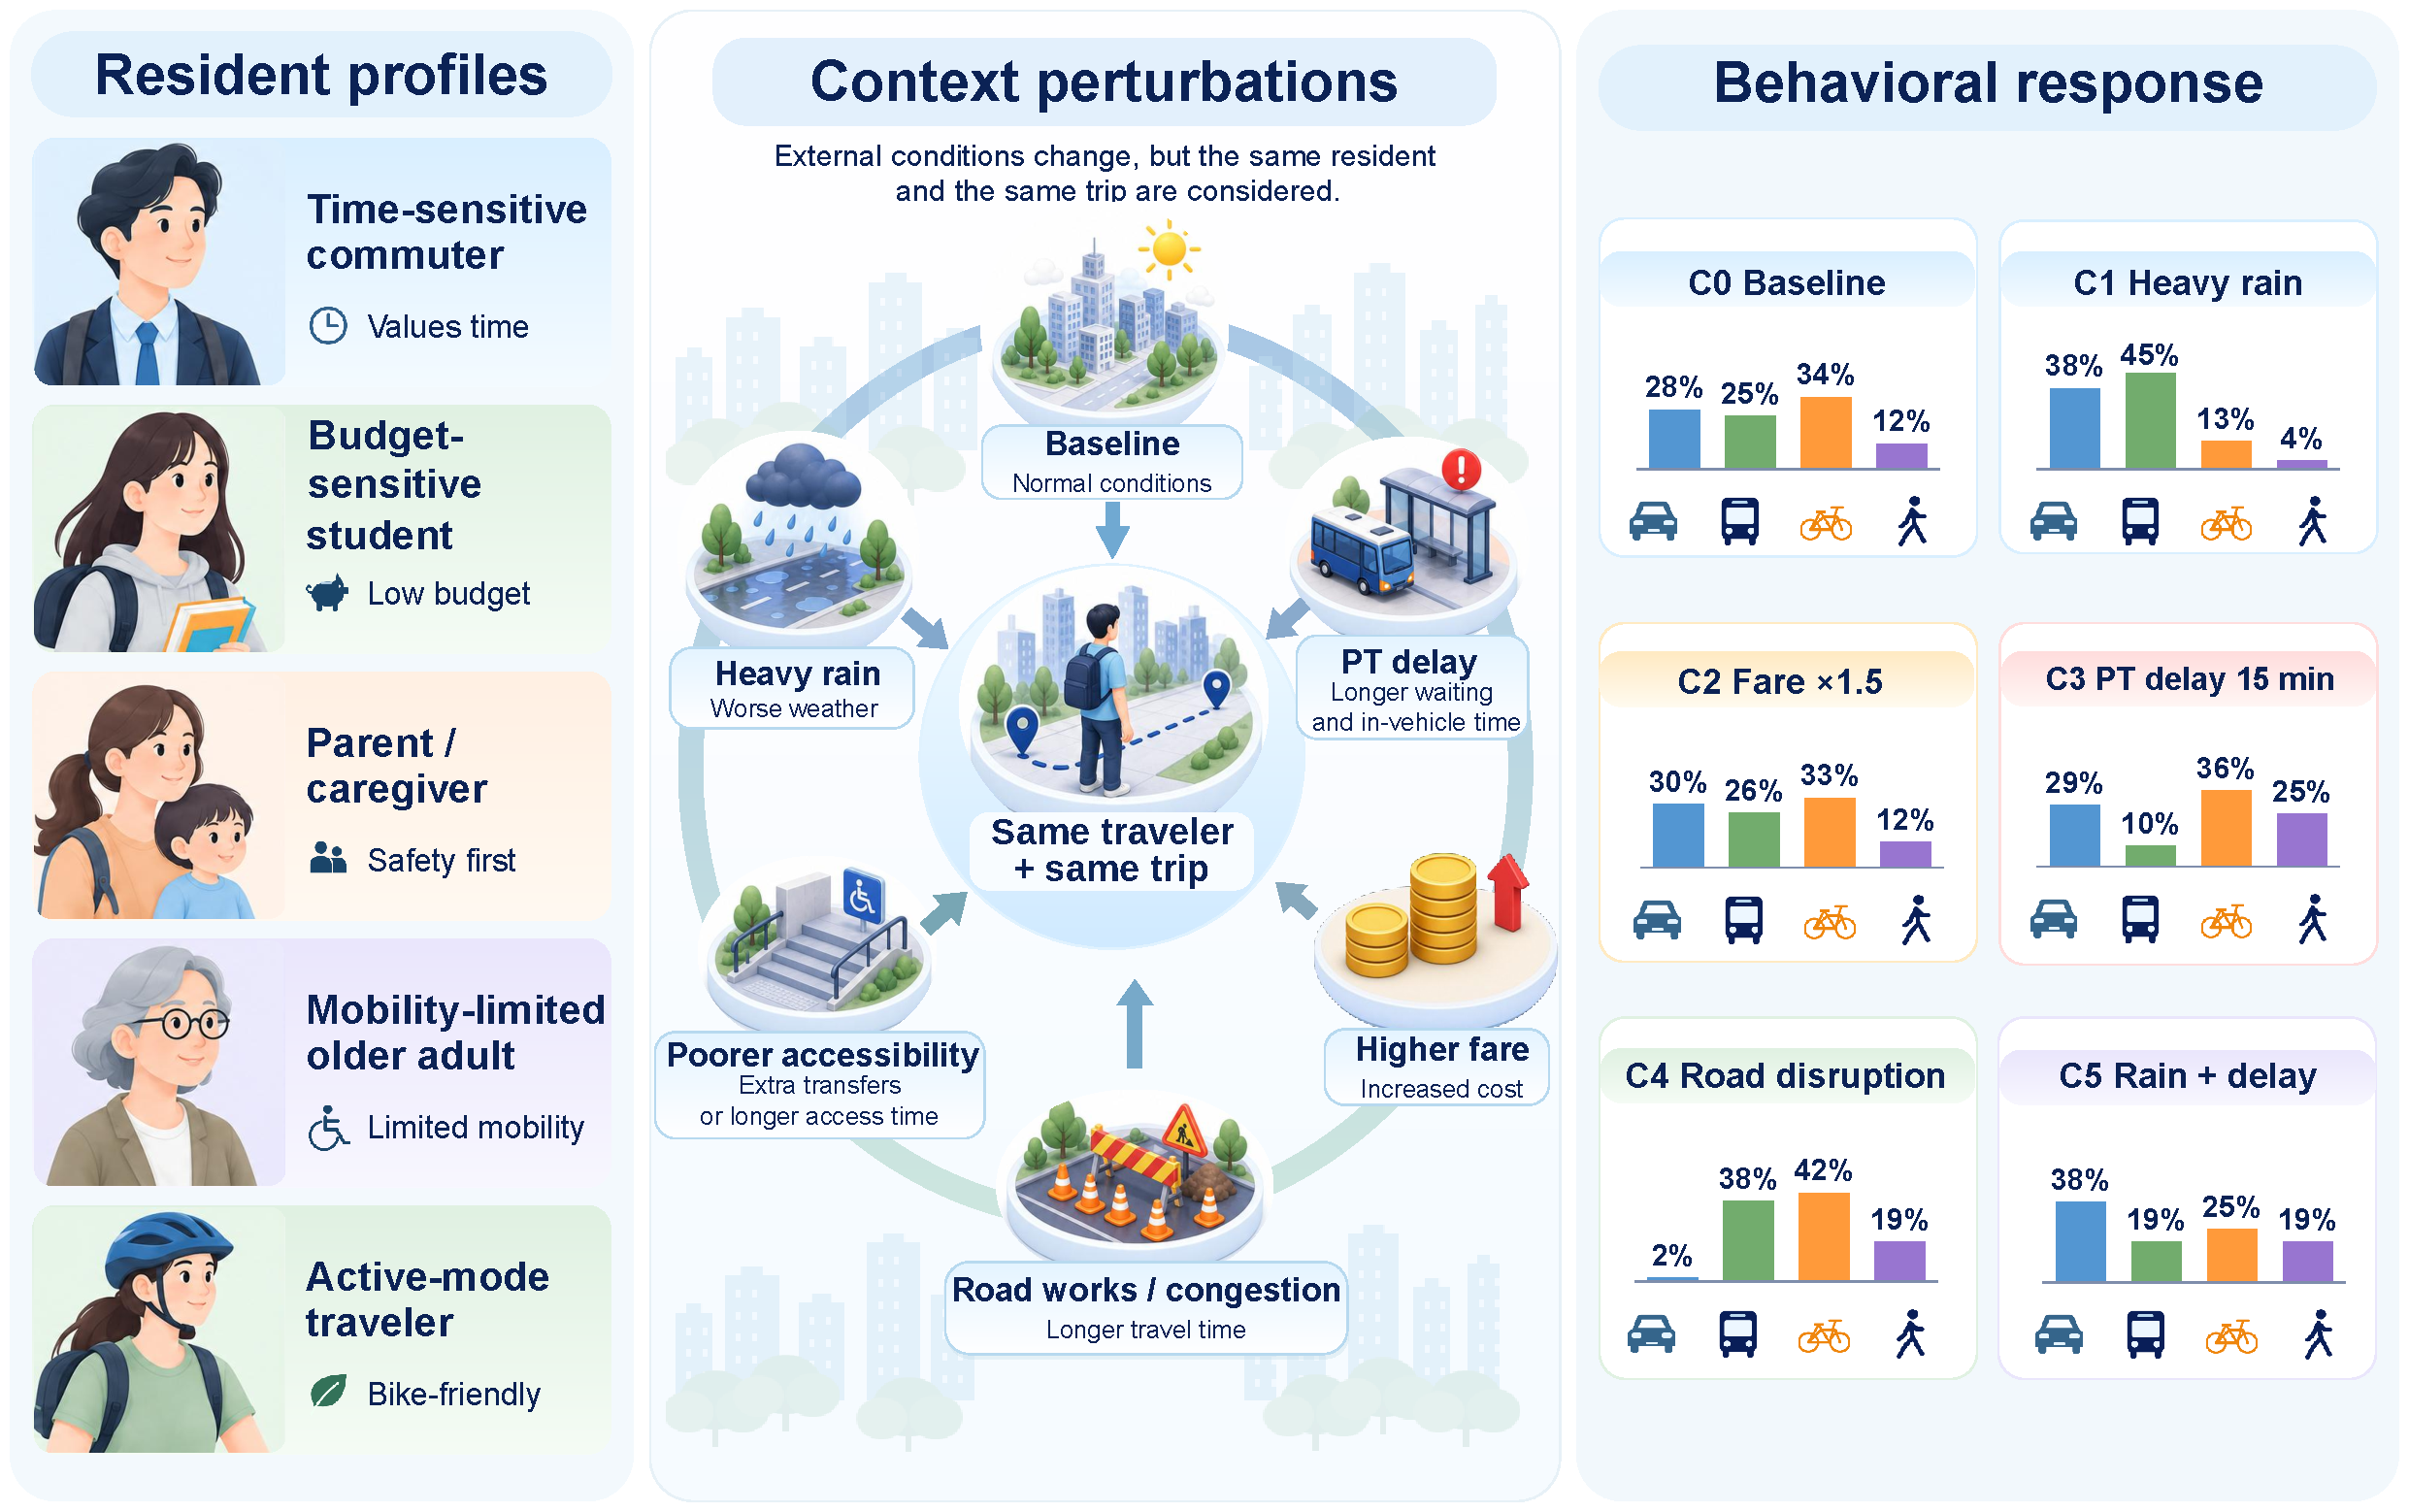
\includegraphics[width=0.95\textwidth,keepaspectratio]{figures/narrative/figure1_response_concept.pdf}
\caption{Traveler--trip pairing and illustrative demand responses. Each pair changes travel conditions while holding the traveler and trip fixed. Profiles are illustrative; bars are rounded, pre-routing mode assignments for 10,000 synthetic Singapore travelers, not survey observations. They use the supply-adapted model defined in Section~\ref{sec:architectures}. Poorer accessibility is evaluated separately. Scenario definitions and exact shares are in Supplementary Table~\ref{supp-tab:singapore}.}
\label{fig:concept}
\end{figure}

Preserving a Teacher's response is only the first test. An LLM can differ from people, and a faithful Student can retain that difference. Research on travel choice and synthetic respondents has already shown why predictive success and plausible language require separate behavioral checks \citep{wang2020deep,martinbaos2023prediction,bisbee2024synthetic,liu2026persona}. A further test arises in simulation: predicted probabilities must become assigned modes, feasible routes and actual boardings. Each step can alter the response. Figure~\ref{fig:concept} illustrates the paired traveler--trip comparison and its connection to aggregate demand.

We examine this chain using matched distillation experiments, stated-choice surveys in Singapore and Shanghai, and controlled network execution in Helsinki. Response supervision is tested against the same archived endpoint targets used by ordinary distillation. A new synthetic-persona experiment examines agreement with a later API model, including a setting where delay-related training examples are withheld. The surveys test the resulting models against people's stated responses. Finally, a four-arm simulation distinguishes a perceived delay from a physical reduction in transit service. These settings provide complementary evidence; they are not a cross-city prediction benchmark.

The findings reveal where a favorable comparison stops carrying over. Response supervision helps within covered tasks, but its advantage reverses on withheld delay scenarios. The Student closest to the archived Teacher can predict the opposite direction to a stated human response. In the network, perceived delay and fewer scheduled trips produce markedly different demand changes. Our contribution is an empirical evaluation of these boundaries and a practical way to locate them. The learning objectives and modular models serve as controlled comparisons within that evaluation, rather than as a claim that a new loss solves behavioral validity.
